\subsection{Localisation}
\label{subsec:models/kf/localisation}
We introduce the map vector $\vec M$ which contains position and feature vectors of $K$ landmarks in our environment.
\begin{align}
	\vec M = 
		\begin{bmatrix}
			\vec m_1 \\
			\vdots \\
			\vec m_K
		\end{bmatrix}
\end{align}
where $\vec m_k$ contains the location and features of the $k^{\text{th}}$ landmark, $\vec m_k \in \mathbb R^d$ and $\vec M \in \mathbb R^{Kd}$. In the localisation problem, we assume $\vec M$ is known and so the graphical model looks as follows:
\begin{figure}[!htb]
\centering
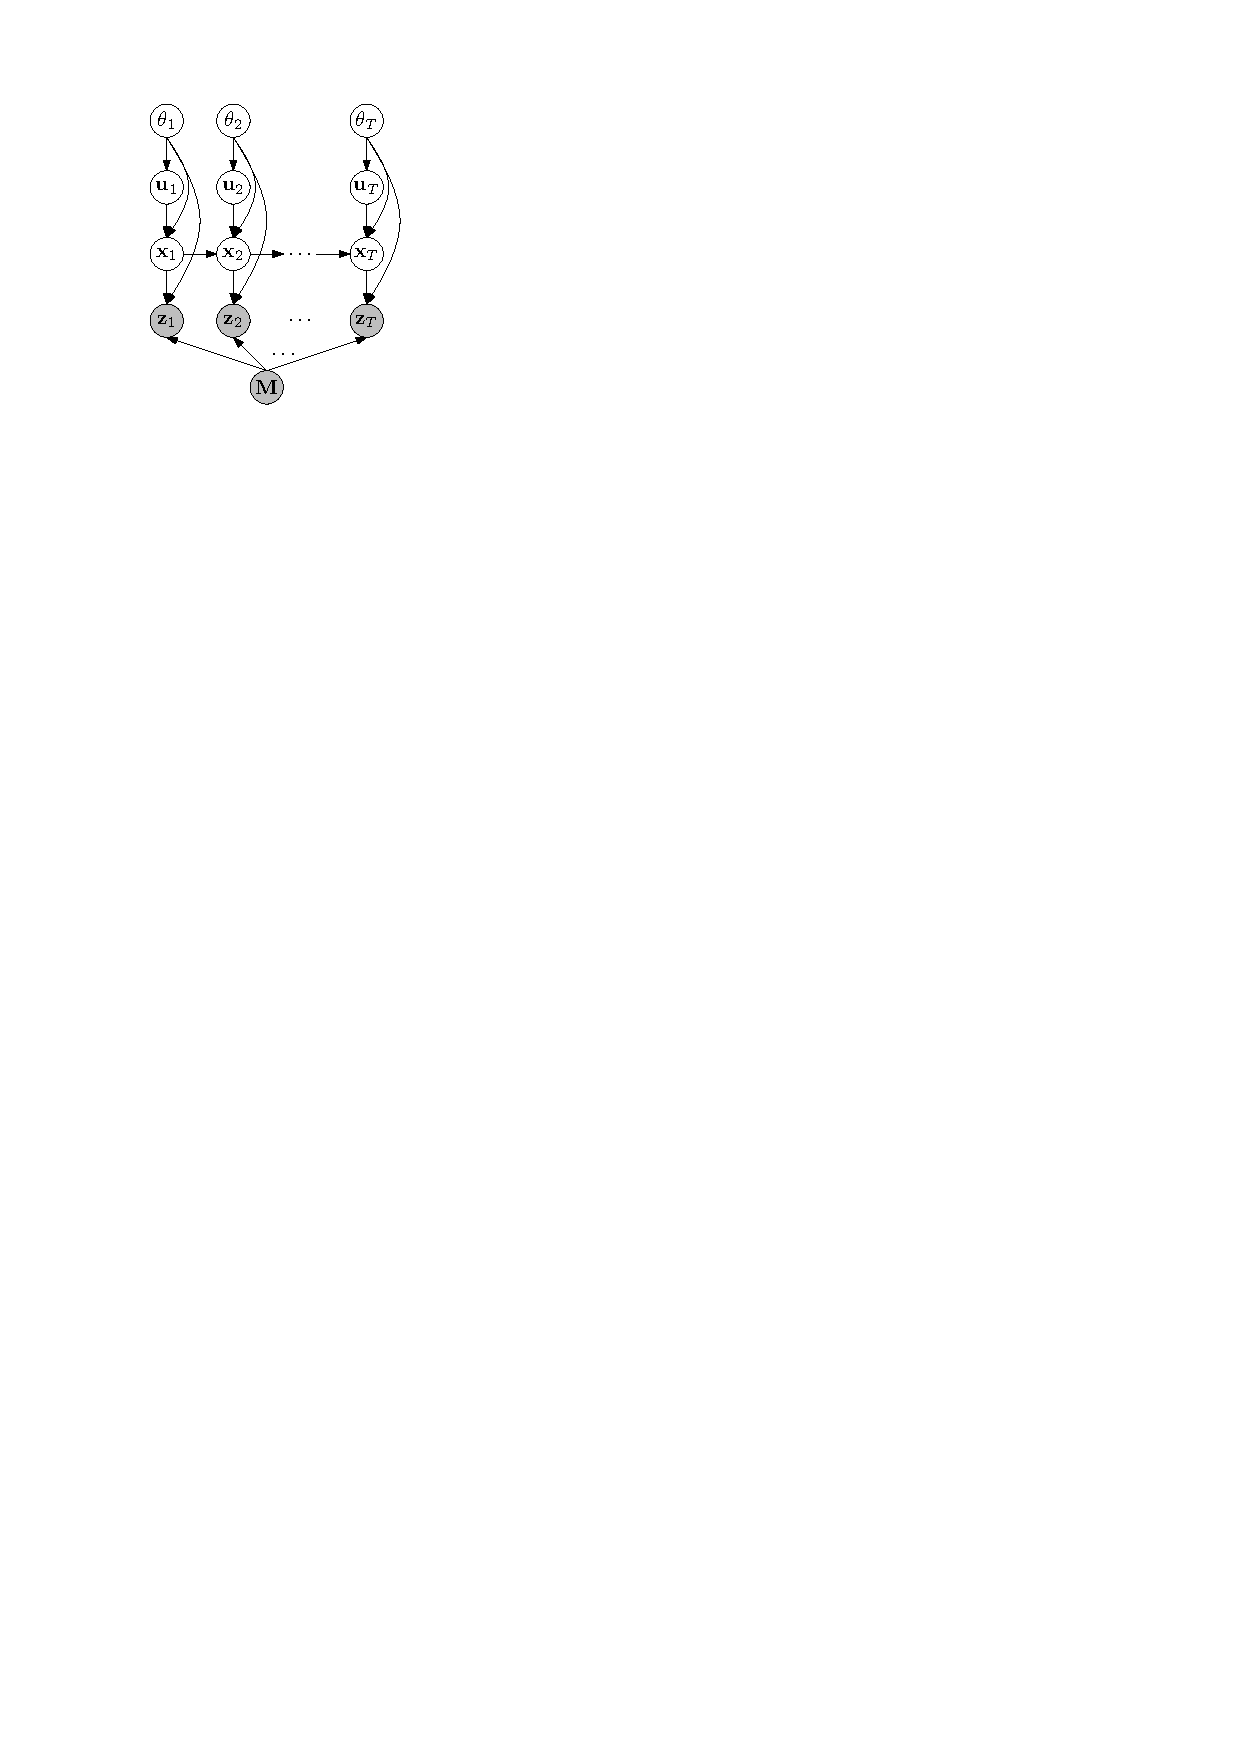
\includegraphics[scale=1]{models/kf/figures/kf-loc}
\caption{Probabilistic Graphical Model for the Kalman Filter for Localisation.}
\label{fig:models/kf/figures/kf-loc}
\end{figure}

The model can be described, for $t = 1, \dotsc, T$, by the following equations:
\begin{align}
	\vec x_t 			&= \vec g(\vec x_{t - 1}, \vec u_t) + \vec \epsilon_t \\
	\vec z_t 			&= \vec h(\vec x_t, \vec u_t, \vec M) + \vec \delta_t \\
	\vec \epsilon_t 	&\sim \Gauss(\vec 0, \vec Q_t) \\
	\vec \delta_t		&\sim \Gauss(\vec 0, \vec R_t)
\end{align}

This model almost exactly resembles the Extended Kalman filter. The update and prediction equations only differ in that
$\vec H_t \triangleq \frac{\partial \vec h(\vec x, \vec u, \vec M)}{\partial \vec x}$ instead of $\vec H_t \triangleq \frac{\partial \vec h(\vec x, \vec u)}{\partial \vec x}$ (evaluated at $\vec x = \vec \mu_{t \mid t - 1}$). We need to characterise $\vec g$ and $\vec h$ to fully describe the EKF algorithm.

\subsubsection{The transition model}
The transition model is defined for the state
\begin{align}
	\vec x_t = 
		\begin{bmatrix}
			x_t \\
			y_t \\
			\theta_t
		\end{bmatrix}
\end{align}
which contains the position and orientation of the vehicle (note the slightly overloaded notation of $\vec x_t$ and $x_t$). The transition model is then described by
\begin{align}
	\vec g(\vec x_{t - 1}, \vec u_t) = \vec x_{t - 1} + 
		\begin{bmatrix}
			-\frac{v_t}{\omega_t} \sin(\theta_{t - 1}) + \frac{v_t}{\omega_t} \sin(\theta_{t - 1} + \omega_t \Delta t) \\
			\frac{v_t}{\omega_t} \cos(\theta_{t - 1}) - \frac{v_t}{\omega_t} \cos(\theta_{t - 1} + \omega_t \Delta t) \\
			\omega_t \Delta t
		\end{bmatrix}
\end{align}
where $\vec u_t = (v_t, \omega_t)^T$ contains translational and rotational velocities.

\subsubsection{The observation model}
\label{subsubsec:models/kf/localisation/obs}
The observation model is defined for the observation
\begin{align}
	\vec z_t = 
		\begin{bmatrix}
			\vec z_{t, 1} \\
			\vdots \\
			\vec z_{t, L}
		\end{bmatrix} \label{eqn:models/kf/localisation/obs}
\end{align}
which contains $L \leq K$ observations $\vec z_{t, 1}, \dotsc, \vec z_{t, L}$ corresponding to the $L$ landmarks observed (out of the total $K$ landmarks) at time $t$. In the simplified case, $\vec z_{t, \ell} = (r_{t, \ell}, \phi_{t, \ell})^T$ contains the Euclidean and angular distance from the landmark. We assume that we know which one out of the $K$ it is by introducing the correspondence variables $\vec c_t$, where if $c_{t, \ell} = j \in \{1, \dotsc, K\}$ then the $i$-th feature observed at $t$, $\vec z_{t, \ell}$, corresponds to the $j$-th landmark, $\vec m_j$. We assume that a landmark $\vec m_j = (m_{j, x}, m_{j, y})^T$ just contains the position of the landmark in this simplified case. Hence we can write, given that $c_{t, \ell} = j$,
\begin{align}
	\vec z_{t, \ell} &= 
						\begin{bmatrix}
							r_{t, \ell} \\
							\phi_{t, \ell}
						\end{bmatrix} 
						+
						\begin{bmatrix}
							\Gauss(0, \sigma^2_r) \\
							\Gauss(0, \sigma^2_\phi)
						\end{bmatrix} \\
					&= 
						\begin{bmatrix}
							\|\vec m_j - (x_t, y_t)^T\| \\
							\arctan\left((m_{j, y} - y_t) / (m_{j, x} - x_t) \right) - \theta_t
						\end{bmatrix}
						+
						\begin{bmatrix}
							\Gauss(0, \sigma^2_r) \\
							\Gauss(0, \sigma^2_\phi)
						\end{bmatrix} \label{eqn:models/kf/localisation/obs2}
\end{align}
The observation model is then described by
\begin{align}
	\vec h(\vec x_t, \vec u_t, \vec M) =
									\begin{bmatrix}
										\|\vec m_{c_{t, 1}} - (x_t, y_t)^T\| \\
										\arctan\left((m_{c_{t, 1}, y} - y_t) / (m_{c_{t, 1}, x} - x_t) \right) - \theta_t \\
										\vdots \\
										\|\vec m_{c_{t, \ell}} - (x_t, y_t)^T\| \\
										\arctan\left((m_{c_{t, \ell}, y} - y_t) / (m_{c_{t, \ell}, x} - x_t) \right) - \theta_t \\
										\vdots \\
										\|\vec m_{c_{t, L}} - (x_t, y_t)^T\| \\
										\arctan\left((m_{c_{t, L}, y} - y_t) / (m_{c_{t, L}, x} - x_t) \right) - \theta_t
									\end{bmatrix}
\end{align}
and
\begin{align}
	\vec R_t = \diag(\sigma^2_r, \sigma^2_\phi, \dotsc, \sigma^2_r, \sigma^2_\phi) \in \mathbb R^{2L \times 2L}
\end{align}